\documentclass[a4paper, 12pt]{article}
\usepackage{fancyhdr}
\usepackage{xcolor}
\usepackage{hyperref}
\usepackage{geometry}
\usepackage{tikz}
\usepackage{graphicx}
\usepackage{caption}
\usepackage{subcaption}
\usepackage{afterpage}
\usepackage{longtable}
\usepackage{booktabs}

\geometry{a4paper, margin=1in}

\definecolor{headerblue}{HTML}{00008B}
\definecolor{white}{HTML}{FFFFFF}
\definecolor{mylinkcolor}{HTML}{8b0000}
\definecolor{myurlcolor}{HTML}{8b0000}

\pagestyle{fancy}
\fancyhf{}

% Header
\fancyhead[L]{
    \begin{tikzpicture}[remember picture, overlay]
        \node[anchor=north west, inner sep=0pt, yshift=1cm] at (current page.north west) {
\includegraphics[height=1cm]{image_head.png}}; % Adjusted height
        \fill[headerblue] (current page.north west) rectangle ([yshift=-1cm]current page.north east);
    \end{tikzpicture}
}

% Footer
\fancyfoot[C]{
    \begin{tikzpicture}[remember picture, overlay]
        \fill[headerblue] (current page.south west) rectangle ([yshift=1cm]current page.south east);
        \node[anchor=south, yshift=0.25cm] at (current page.south) {\color{white}\bfseries\thepage};
    \end{tikzpicture}
}

\renewcommand{\headrulewidth}{0pt}
\renewcommand{\footrulewidth}{0pt}

% Title
\title{\Huge\textbf{\textcolor{headerblue}{Pentests Results}}}
\author{}
\date{}

% Adjust the style of sections (including \section*)
\usepackage{titlesec}
\titleformat{\section}[hang]{\Huge\bfseries\color{headerblue}}{}{0em}{}

% Hyperlink setup
\hypersetup{
    colorlinks=true,
    linkcolor=mylinkcolor,
    filecolor=magenta,
    urlcolor=myurlcolor,
}

\begin{document}
\maketitle
\thispagestyle{fancy}

% Adjust the vertical space after the title. Experiment with this value.
\vspace{-1em} 

% Add "Charts" title and charts on the same page
\afterpage{\aftergroup\restoregeometry % Restore geometry immediately after the page
    \thispagestyle{fancy} % Apply the fancy style to the blank page
    
    % Add "Charts" title and include both charts in a single figure environment
    \begin{figure}[htbp]
        \centering
        
        \begin{subfigure}{\textwidth} % Full width for the subfigures
            \centering
            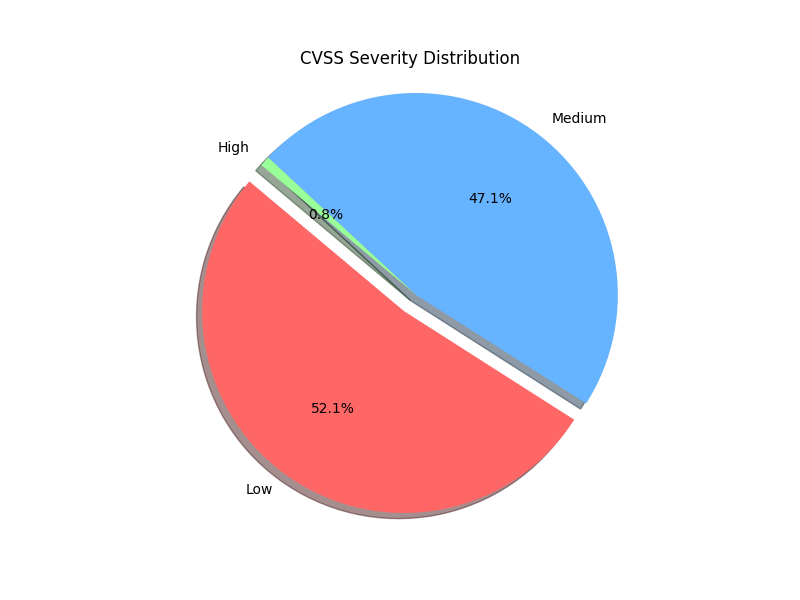
\includegraphics[width=0.9\linewidth]{alvo_pie_chart.png} % Adjust width of image as needed
            \caption{Figure 1: Pie Chart}
        \end{subfigure}
        
        \vspace{0.5cm} % Adjust vertical space between subfigures
        
        \begin{subfigure}{\textwidth} % Full width for the subfigures
            \centering
            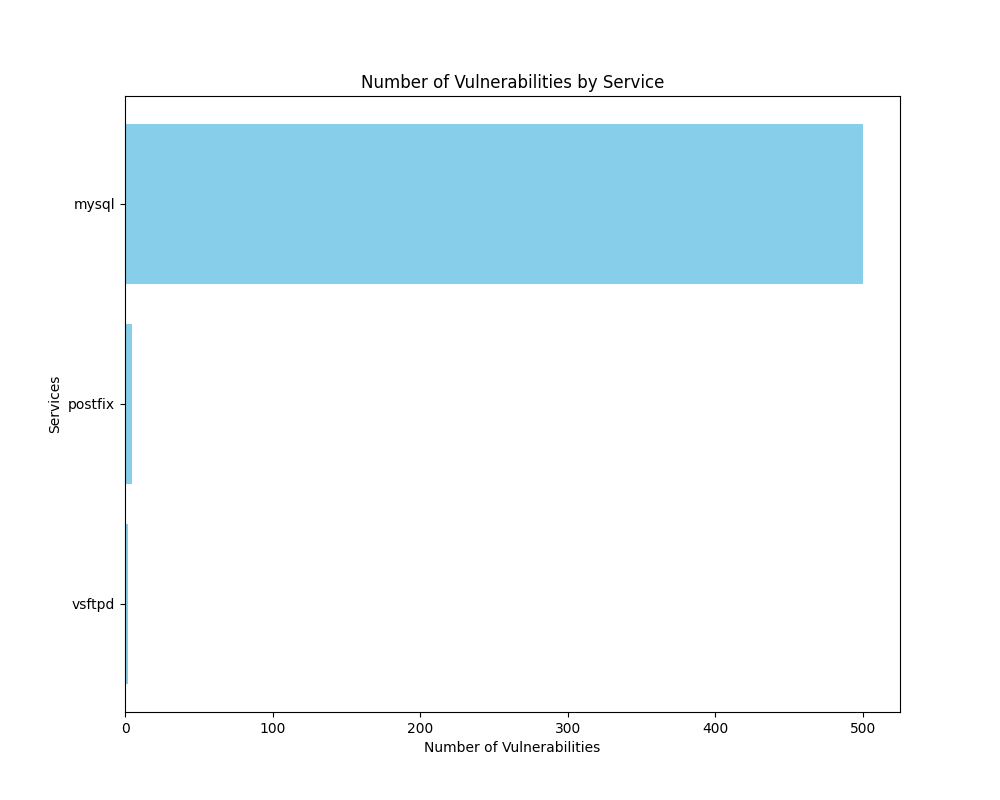
\includegraphics[width=0.9\linewidth]{alvo_bar_chart.png} % Adjust width of image as needed
            \caption{Figure 2: Bar Chart}
        \end{subfigure}
    \end{figure}
    \restoregeometry % Restore normal geometry settings
}

$body$


\end{document}